% THIS IS SIGPROC-SP.TEX - VERSION 3.1
% WORKS WITH V3.2SP OF ACM_PROC_ARTICLE-SP.CLS
% APRIL 2009
%
% It is an example file showing how to use the 'acm_proc_article-sp.cls' V3.2SP
% LaTeX2e document class file for Conference Proceedings submissions.
% ----------------------------------------------------------------------------------------------------------------
% This .tex file (and associated .cls V3.2SP) *DOES NOT* produce:
%       1) The Permission Statement
%       2) The Conference (location) Info information
%       3) The Copyright Line with ACM data
%       4) Page numbering
% ---------------------------------------------------------------------------------------------------------------
% It is an example which *does* use the .bib file (from which the .bbl file
% is produced).
% REMEMBER HOWEVER: After having produced the .bbl file,
% and prior to final submission,
% you need to 'insert'  your .bbl file into your source .tex file so as to provide
% ONE 'self-contained' source file.
%
% Questions regarding SIGS should be sent to
% Adrienne Griscti ---> griscti@acm.org
%
% Questions/suggestions regarding the guidelines, .tex and .cls files, etc. to
% Gerald Murray ---> murray@hq.acm.org
%
% For tracking purposes - this is V3.1SP - APRIL 2009

\documentclass{dependencies/acm_proc_article-sp}

\usepackage{url}
\usepackage{color}
\usepackage{verbatim}
\usepackage{listings}
\lstset{
  language=C++,             % choose the language of the code
  basicstyle=\small,       % the size of the fonts that are used for the code
  numbers=left,                   % where to put the line-numbers
  numberstyle=\footnotesize,      % the size of the fonts that are used for the line-numbers
  stepnumber=0,                   % the step between two line-numbers. If it is 1 each line will be numbered
  numbersep=5pt,                  % how far the line-numbers are from the code
  backgroundcolor=\color{white},  % choose the background color. You must add \usepackage{color}
  showspaces=false,               % show spaces adding particular underscores
  showstringspaces=false,         % underline spaces within strings
  showtabs=false,                 % show tabs within strings adding particular underscores
  %frame=single,                   % adds a frame around the code
  tabsize=2,              % sets default tabsize to 2 spaces
  captionpos=t,                   % sets the caption-position to bottom
  breaklines=false,        % sets automatic line breaking
  breakatwhitespace=false,    % sets if automatic breaks should only happen at whitespace
  escapeinside={\%}{)}          % if you want to add a comment within your code
}


\begin{document}

\title{ Development Of Parallel Matrix Operations }
%
% You need the command \numberofauthors to handle the 'placement
% and alignment' of the authors beneath the title.
%
% For aesthetic reasons, we recommend 'three authors at a time'
% i.e. three 'name/affiliation blocks' be placed beneath the title.
%
% NOTE: You are NOT restricted in how many 'rows' of
% "name/affiliations" may appear. We just ask that you restrict
% the number of 'columns' to three.
%
% Because of the available 'opening page real-estate'
% we ask you to refrain from putting more than six authors
% (two rows with three columns) beneath the article title.
% More than six makes the first-page appear very cluttered indeed.
%
% Use the \alignauthor commands to handle the names
% and affiliations for an 'aesthetic maximum' of six authors.
% Add names, affiliations, addresses for
% the seventh etc. author(s) as the argument for the
% \additionalauthors command.
% These 'additional authors' will be output/set for you
% without further effort on your part as the last section in
% the body of your article BEFORE References or any Appendices.

\numberofauthors{3} %  in this sample file, there are a *total*
% of EIGHT authors. SIX appear on the 'first-page' (for formatting
% reasons) and the remaining two appear in the \additionalauthors section.
%
\author{
% You can go ahead and credit any number of authors here,
% e.g. one 'row of three' or two rows (consisting of one row of three
% and a second row of one, two or three).
%
% The command \alignauthor (no curly braces needed) should
% precede each author name, affiliation/snail-mail address and
% e-mail address. Additionally, tag each line of
% affiliation/address with \affaddr, and tag the
% e-mail address with \email.
%
% 1st. author
\alignauthor
Nicholas Dexter \\
       \affaddr{RIT}\\
       \email{nxd3734@rit.edu}
% 2nd. author
\alignauthor
Brian Gianforcaro \\
       \affaddr{RIT}\\
       \email{bjg1955@rit.edu}
% 3rd. author
\alignauthor
Jerome Marhic \\
       \affaddr{RIT}\\
       \email{jxm2644@rit.edu}
}
\maketitle
\begin{abstract}
%the formatting guidelines for ACM SIG Proceedings.
%It complements the document \textit{Author's Guide to Preparing
%ACM SIG Proceedings Using \LaTeX$2_\epsilon$\ and Bib\TeX}. This
%source file has been written with the intention of being
%compiled under \LaTeX$2_\epsilon$\ and BibTeX.
%
%The developers have tried to include every imaginable sort
%of ``bells and whistles", such as a subtitle, footnotes on
%title, subtitle and authors, as well as in the text, and
%every optional component (e.g. Acknowledgments, Additional
%Authors, Appendices), not to mention examples of
%equations, theorems, tables and figures.
%
%To make best use of this sample document, run it through \LaTeX\
%and BibTeX, and compare this source code with the printed
%output produced by the dvi file.

A Parallel Matrix Manipulation Library (PMML) is presented for use on sequential and symmetric multiprocessing (SMP) systems. PMML is written using the Parallel Java library developed by Professor Alan Kaminsky at the Rochester Institute of Technology. PMML provides methods for the following operations: matrix-vector multiplication, matrix-matrix multiplication, and matrix inversion and solution to the linear system $A x=b$. An implementation of the Strassen algorithm for efficient matrix multiplication is provided for use sequentially and on SMP systems. Gaussian elimination with partial-pivoting is used to find the row-reduced form of the matrix $A$ and backsubstitution is used to solve the linear system. Algorithms for sequential solution and parallel solution on SMP systems are provided. Performance metrics are presented to compare the {\em speedup} and {\em sizeup} gained in the parallel over the sequential versions.
\end{abstract}

%% A category with the (minimum) three required fields
%\category{H.4}{Information Systems Applications}{Miscellaneous}
%%%A category including the fourth, optional field follows...
%
%\terms{Theory}

\keywords{ Parallel Matrix Manipulation Library, PMML, Parallel Java, PJ, Strassen algorithm, Gaussian elimination, RIT } % NOT required for Proceedings
%
%\footnotetext[1]{NoSQL databases, also known as structured storage are known for not requiring a fixed table schema and often avoid join operations. The thing that
% links them together is there use of alternate query languages from SQL.}

\section{Introduction}
\subsection{Numerical Linear Algebra}

The use of computers to manipulate and solve matrices has found many applications in computer science, finances, engineering, biology, and physics \cite{TrefethenNLA}. Since many problems can be reduced to a system of linear equations, particularly in the solution of differential equations as seen in many examples in the Matrix Market maintained by NIST \cite{MatrixMarket}, numerical linear algebra has become increasingly useful in the study of such systems. In the High Performance Computing (HPC) world, a large amount of effort and resources have been devoted to developing toolsets that allow these problems to be solved in parallel \cite{SCALAPACK,LAPACK,PLASMA,PSBLAS}.

Since its development in 1979, the {\em de facto} standard for basic linear algebra operations has been the Basic Linear Algebra Subprograms (BLAS) \cite{BLAS}. Most modern implementations of numerical linear algebra libraries still rely on this toolset written in FORTRAN90 \cite{LAPACK}, though other language implementations exist \cite{CLAPACK,JBLAS}. Early in the applications of computers to such problems, vector computers reigned supreme in numerical linear algebra due to their ability to apply operations to one-dimensional arrays of data. As scalar processors became cheaper and more readily available, a trend began of using large networks of scalar processors to perform parallel operations. This trend continues today as we see some of the largest HPCs are based off of this model \cite{Jaguar}.

While there are some leaders in the pack of toolsets providing an easily accessible parallel implementation of the standard BLAS \cite{SCALAPACK,PLAPACK}, no clear winner has emerged. The PMML does not attempt to challenge these toolsets, as such a challenger would be many years in development, but serves as an educational exercise in developing basic matrix manipulation methods in parallel. 

\subsection{Parallel Matrix Operations}

The process of fitting more and more cores onto a single die is now leading us to consumer systems with multi-core chips. Since these systems share the symmetric multiprocessing model, these types of systems and larger SMP systems are the ideal target for the Parallel Matrix Manipulation Library (PMML). The PMML uses Parallel Java as a backbone to acheive the desired parallelism by dividing up computation in the agenda parallelism scheme.

By dividing up the operations of multiplying slices of matrices among processors, a clear advantage is gained in terms of overall computation time. For the parallel version of the Strassen algorithm, the task of computing the block submatrices is divided among threads to achieve a reduced runtime. In the case of Gaussian elimination with partial-pivoting, the elementary row operations performed to reduce the matrix to row-echelon form are parallelized to achieve the desired speedup.

\section{Methods}

\begin{verbatim}
MatrixInt A = ...
VectorInt B = ...
Matrix C = MatrixOp.mult(A,B)
Matrix C = MatrixParallelOp.mult(A,B)

\end{verbatim}



\subsection{Matrix-Matrix Multiplication}

\subsubsection{Classic matrix multiplication}
%Matrices of the form $A_{\mbox{\tiny m}\scriptscriptstyle\times\mbox{\tiny n}}$, where $m$ is the number of rows and $n$ is the number of columns.
The Parallel Matrix Manipulation Library provides two methods for the multiplication of matrices of the form $A_{\mbox{\tiny m,n}}$, where $m$ is the number of rows and $n$ is the number of columns. The first of which is classic matrix multiplication of the form
\begin{equation}
\label{AB=C}
A_{\mbox{\tiny m,n}}\cdot B_{\mbox{\tiny n,p}} = C_{\mbox{\tiny m,p}}
\end{equation}
where the product of an $m\times n$ matrix and a $n\times p$ matrix is an $m\times p$ matrix.

In the PMML, the following code:
\begin{verbatim}
Matrix C = MatrixOp.mult(A,B);
Matrix C = MatrixParallelOp.mult(A,B);
\end{verbatim}
returns the product $C=AB$, using the sequential and parallel algorithms respectively. Note that the operation is valid only if the number of columns of $A$ equals the number of rows of $B$, otherwise an Exception is thrown.

The matrix multiplication is performed by multiplying each row of $A$ by each column of $B$ \cite{MatrixMultiplication}. Sequentially, one thread performs all the operations by looping on every row of $A$ and every column of $B$. The complexity is in $O(m\cdot n\cdot p)$ if $A$ and $B$ are rectangular matrices of size $m\times n$ and $n\times p$ respectively. This method is easily parallelizable over several threads; each thread computing a range of rows of $A$. The complexity is then $O( \frac{m}{K}\cdot n\cdot p )$, $K$ being the number of threads used.

\subsubsection{Strassen matrix multiplication}
The Parallel Matrix Manipulation Library also provides an implementation of the Strassen algorithm, an algorithm discovered by Volker Strassen that is $O( n^{2.807})$ \cite{StrassenAlgorithm}.

Let $A$, $B$ be two real valued square matrices of size $2^n\times2^n$ for some $n$. If they are not this size, the missing rows and columns must be filled with zeros. In order to divide the computation, $A$, $B$ and $C$ are partitioned into equally sized blocks,
\begin{equation*}
\label{StrassenBlocks}
\mathbf{A} = \begin{bmatrix} \mathbf{A}_{1,1} & \mathbf{A}_{1,2} \\ \mathbf{A}_{2,1} & \mathbf{A}_{2,2} \end{bmatrix}
\mbox { , }
\mathbf{B} = \begin{bmatrix} \mathbf{B}_{1,1} & \mathbf{B}_{1,2} \\ \mathbf{B}_{2,1} & \mathbf{B}_{2,2} \end{bmatrix}
\mbox { , }
\mathbf{C} = \begin{bmatrix} \mathbf{C}_{1,1} & \mathbf{C}_{1,2} \\ \mathbf{C}_{2,1} & \mathbf{C}_{2,2} \end{bmatrix}
\end{equation*}
with each $\mathbf{A}_{i,j}, \mathbf{B}_{i,j}, \mathbf{C}_{i,j}$ of size $2^{n-1} \times 2^{n-1}$. With this partitioning, the matrix $C$ can be expressed as the blocks
\begin{eqnarray*}
\mathbf{C}_{1,1} = \mathbf{A}_{1,1}\cdot \mathbf{B}_{1,1} + \mathbf{A}_{1,2}\cdot \mathbf{B}_{2,1},\\
\mathbf{C}_{1,2} = \mathbf{A}_{1,1}\cdot \mathbf{B}_{1,2} + \mathbf{A}_{1,2}\cdot \mathbf{B}_{2,2},\\
\mathbf{C}_{2,1} = \mathbf{A}_{2,1}\cdot \mathbf{B}_{1,1} + \mathbf{A}_{2,2}\cdot \mathbf{B}_{2,1},\\
\mathbf{C}_{2,2} = \mathbf{A}_{2,1}\cdot \mathbf{B}_{1,2} + \mathbf{A}_{2,2}\cdot \mathbf{B}_{2,2}.
\end{eqnarray*}
In the case of standard matrix multiplication, the partitioning of $C$ in this way yields a total of 8 matrix multiplications. By introducing the following matrices
\begin{align*}
&\mathbf{M}_{1} := (\mathbf{A}_{1,1} + \mathbf{A}_{2,2})\cdot (\mathbf{B}_{1,1} + \mathbf{B}_{2,2}),\\
&\mathbf{M}_{2} := (\mathbf{A}_{2,1} + \mathbf{A}_{2,2})\cdot \mathbf{B}_{1,1},\\
&\mathbf{M}_{3} := \mathbf{A}_{1,1}\cdot (\mathbf{B}_{1,2} - \mathbf{B}_{2,2}),\\
&\mathbf{M}_{4} := \mathbf{A}_{2,2}\cdot (\mathbf{B}_{2,1} - \mathbf{B}_{1,1}),\\
&\mathbf{M}_{5} := (\mathbf{A}_{1,1} + \mathbf{A}_{1,2})\cdot \mathbf{B}_{2,2},\\
&\mathbf{M}_{6} := (\mathbf{A}_{2,1} - \mathbf{A}_{1,1})\cdot (\mathbf{B}_{1,1} + \mathbf{B}_{1,2}),\\
&\mathbf{M}_{7} := (\mathbf{A}_{1,2} - \mathbf{A}_{2,2})\cdot (\mathbf{B}_{2,1} + \mathbf{B}_{2,2}).
\end{align*}
and then computing 
\begin{align*}
&\mathbf{C}_{1,1} = \mathbf{M}_{1} + \mathbf{M}_{4} - \mathbf{M}_{5} + \mathbf{M}_{7}\\
&\mathbf{C}_{1,2} = \mathbf{M}_{3} + \mathbf{M}_{5}\\
&\mathbf{C}_{2,1} = \mathbf{M}_{2} + \mathbf{M}_{4}\\
&\mathbf{C}_{2,2} = \mathbf{M}_{1} - \mathbf{M}_{2} + \mathbf{M}_{3} + \mathbf{M}_{6}
\end{align*}
we see that the total number of matrix partition multiplications drops from $8$ to $7$. Since these matrix multiplications are more costly than matrix additions and subtractions, efficiency is gained in the computation of $C$.

The idea consists in recursively dividing both matrices into 4 smaller square matrices, until those submatrices degenerate into numbers, that is have a size of 1, and replace the last multiplication by the sum of 18 submatrices. However, by padding with zeroes the matrices to the closest power of 2, we can multiply matrices of any size. Due to this recursive nature, this algorithm is not easily parallelizable but we managed to parallelize the first step before the recursion to obtain speedups with up to 7 threads (see results section).

In the PMML, the following code:

{\tt Matrix C = MatrixOp.strassenMult(A,B);\\
Matrix C = MatrixParallelStr.mult(A,B);}

returns the product $C=AB$, using the sequential and parallel versions respectively of the Strassen algorithm. 

\subsection{Matrix-Vector Multiplication}

Describe the problem of matrix-vector multiplication and introduce the terms.

\subsection{Solution to Linear Systems of Equations}

To solve a linear system of equations of the form $Ax=b$, where $A$ is an $m\times n$ matrix, $b$ is an $m\times 1$ vector, and $x$ is the $m\times 1$ solution vector, first the matrix must be inverted. For most matrices, this presents a problem, as the inverse of a matrix is generally not easy to compute and may not even exist. Gaussian elimination is the process of performing a series of elementary row operations to the matrix $A$ to reduce it to a form, known as row-echelon form, that can be easily inverted.

\section{Results}

\subsection{Matrix-Vector Multiplication}

\begin{center}
\begin{tabular}{|r|r|r|r|r|r|r|}\hline
{\em n} & {\em K} & {\em T (msec)} & {\em Speedup} & {\em Eff} & {\em EDSF} \\\hline
1000    & seq     &  22        & xxxxx       & xxxxx   & xxxxx     \\\hline
1000    & 1       &  47        & 0.468       & 0.468   & xxxxx     \\\hline
1000    & 2       &  40        & 0.550       & 0.275   & 0.702     \\\hline
1000    & 4       &  34        & 0.647       & 0.162   & 0.631     \\\hline
1000    & 8       &  35        & 0.629       & 0.079   & 0.708     \\\hline
2000    & seq     &  83        & xxxxx       & xxxxx   & xxxxx     \\\hline
2000    & 1       &  90        & 0.922       & 0.922   & xxxxx    \\\hline
2000    & 2       &  35        & 2.371       & 1.186   & -0.222    \\\hline
2000    & 4       &  14        & 5.929       & 1.482   & -0.126    \\\hline
2000    & 8       &   9        & 9.222       & 1.153   & -0.029    \\\hline
4000    & seq     &  338       & xxxxx       & xxxxx   & xxxxx     \\\hline
4000    & 1       &  340       & 0.994       & 0.994   & xxxxx     \\\hline
4000    & 2       &  177       & 1.910       & 0.955   & 0.041     \\\hline
4000    & 4       &  91        & 3.714       & 0.929   & 0.024     \\\hline
4000    & 8       &  34        & 9.941       & 1.243   & -0.029    \\\hline
\end{tabular}
\end{center}

\begin{center}
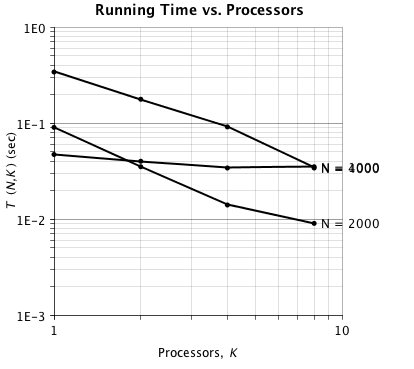
\includegraphics[scale=0.5]{images/matrix-vector/running-vs-proc.png}
\end{center}
\begin{center}
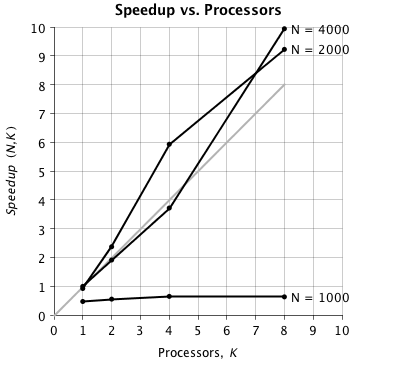
\includegraphics[scale=0.5]{images/matrix-vector/speedup-vs-proc.png}
\end{center}
\begin{center}
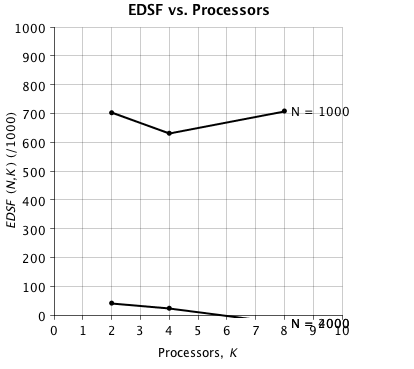
\includegraphics[scale=0.5]{images/matrix-vector/esdf-vs-proc.png}
\end{center}
\begin{center}
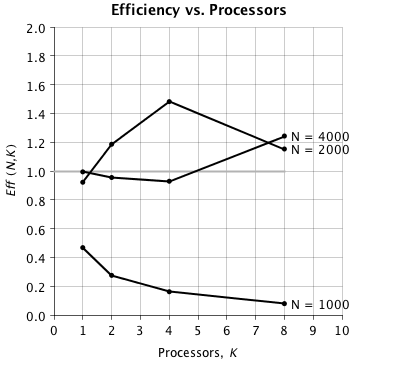
\includegraphics[scale=0.5]{images/matrix-vector/eff-vs-proc.png}
\end{center}


\subsection{Matrix-Matrix Multiplication}

Sequential and Parallel Implementation
\begin{center}
\begin{tabular}{|r|r|r|r|r|r|r|}\hline
{\em n} & {\em K} & {\em T (msec)} & {\em Speedup} & {\em Eff} & {\em EDSF} \\\hline
1000    & seq     &   32609        &   xxx         & xxx       & xxx        \\\hline
1000    & 1       &   53546        & 0.609        & 0.609    & xxx        \\\hline
1000    & 2       &   15812        & 2.062        & 1.031    & -0.409     \\\hline
1000    & 4       &    8101        & 4.025        & 1.006    & -0.132     \\\hline
1000    & 8       &    4703        & 6.934        & 0.991    & -0.064     \\\hline
1000    & 8       &    4210        & 7.746        & 0.968    & -0.053     \\\hline
500     & seq     &    4797        &   xxx         & xxx       & xxx        \\\hline
500     & 1       &    2046        & 2.345         & 2.345     & xxx        \\\hline
500     & 2       &    2632        & 1.823         & 0.911      & 1.573      \\\hline
500     & 4       &    1411        & 3.400         & 0.850     & 0.586      \\\hline
500     & 7       &     953        & 5.034         & 0.719     & 0.377      \\\hline
500     & 8       &     789        & 6.080         & 0.760     & 0.298      \\\hline
100     & seq     &      71        &   xxx         & xxx       & xxx        \\\hline
100     & 1       &      62        & 1.145        & 1.145    & xxx        \\\hline
100     & 2       &      42        & 1.690        & 0.845    & 0.355     \\\hline
100     & 4       &      36        & 1.972        & 0.493    & 0.441     \\\hline
100     & 7       &      35        & 2.029        & 0.290    & 0.492     \\\hline
100     & 8       &      35        & 2.029        & 0.254    & 0.502     \\\hline
\end{tabular}
\end{center}

\begin{center}
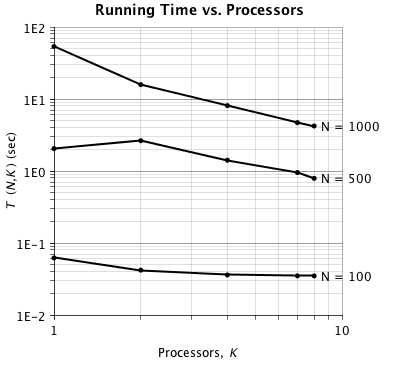
\includegraphics[scale=0.5]{images/parallel/run-vs-proc.png}
\end{center}
\begin{center}
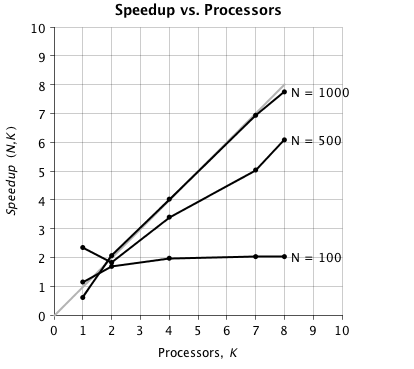
\includegraphics[scale=0.5]{images/parallel/speedup-vs-proc.png}
\end{center}
\begin{center}
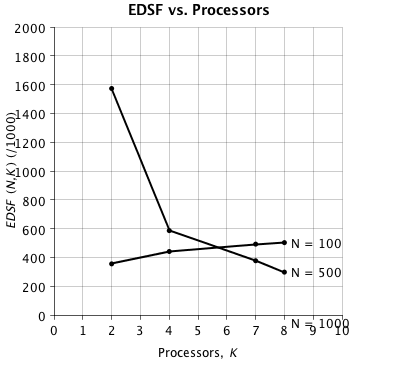
\includegraphics[scale=0.5]{images/parallel/edsf-vs-proc.png}
\end{center}
\begin{center}
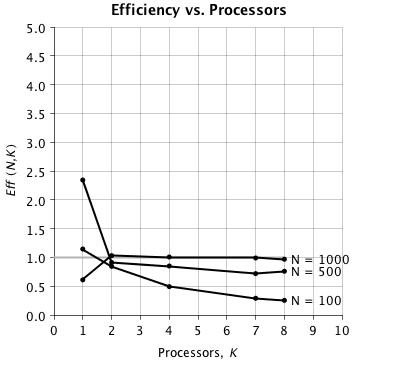
\includegraphics[scale=0.5]{images/parallel/eff-vs-proc.png}
\end{center}


Sequential Strassen and Parallel Strassen Implementation
\begin{center}
\begin{tabular}{|r|r|r|r|r|r|r|}\hline
{\em n} & {\em K} & {\em T (msec)} & {\em Speedup} & {\em Eff} & {\em EDSF} \\\hline
1000    & seq     &   12296           &   xxx         & xxx       & xxx        \\\hline
1000    & 1       &   12105           &   1.016       & 1.016     & xxx        \\\hline
1000    & 2       &   7139            &   1.722       & 0.861     & 0.180      \\\hline
1000    & 4       &   4184            &   2.939       & 0.735     & 0.128      \\\hline
1000    & 8       &   2467            &   4.984       & 0.712     & 0.071      \\\hline
1000    & 8       &   2372            &   5.184       & 0.648     & 0.081      \\\hline
500     & seq     &   1792            &   xxx         & xxx       & xxx        \\\hline
500     & 1       &   1787            &   1.003       & 1.003     & xxx        \\\hline
500     & 2       &   1112            &   1.612       & 0.806     & 0.245      \\\hline
500     & 4       &   713             &   2.513       & 0.628     & 0.199      \\\hline
500     & 7       &   505             &   3.549       & 0.507     & 0.163      \\\hline
500     & 8       &   502             &   3.570       & 0.446     & 0.178      \\\hline
100     & seq     &   71              &   xxx         & xxx       & xxx        \\\hline
100     & 1       &   37              &   1.919       & 1.919     & xxx        \\\hline
100     & 2       &   69              &   1.029       & 0.514     & 2.730      \\\hline
100     & 4       &   70              &   1.014       & 0.254     & 2.189      \\\hline
100     & 7       &   68              &   1.044       & 0.149     & 1.977      \\\hline
100     & 8       &   68              &   1.044       & 0.131     & 1.958      \\\hline
\end{tabular}
\end{center}

\begin{center}
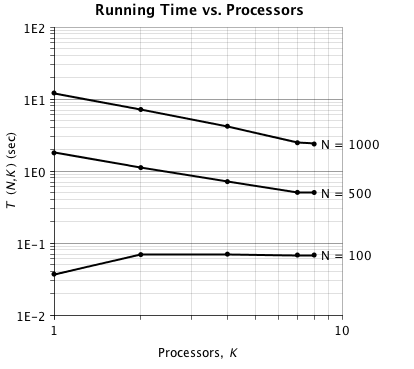
\includegraphics[scale=0.5]{images/parallel-stras/running-vs-proc.png}
\end{center}
\begin{center}
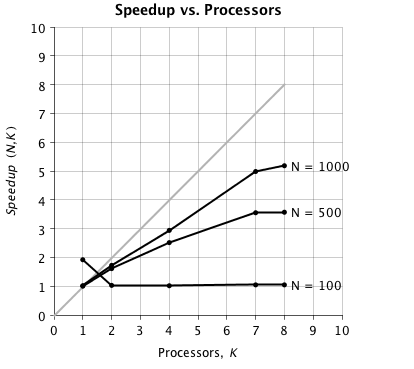
\includegraphics[scale=0.5]{images/parallel-stras/speedup-vs-proc.png}
\end{center}
\begin{center}
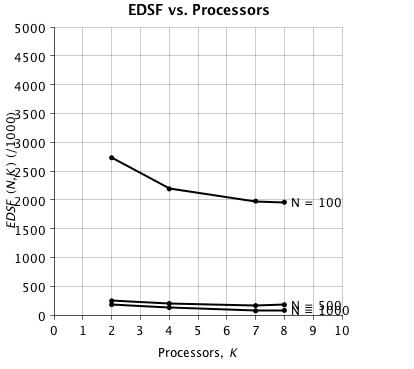
\includegraphics[scale=0.5]{images/parallel-stras/edsf-vs-proc.png}
\end{center}
\begin{center}
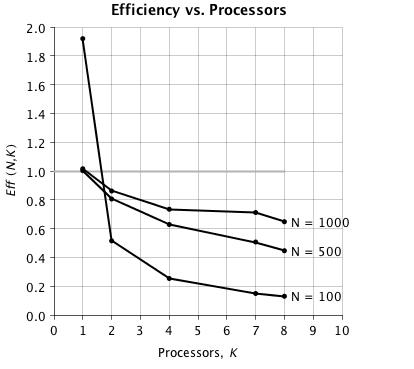
\includegraphics[scale=0.5]{images/parallel-stras/eff-vs-proc.png}
\end{center}


\subsection{Gaussian Elimination and Solution}

\begin{center}
\begin{tabular}{|r|r|r|r|r|r|r|}\hline
{\em n} & {\em K} & {\em T (msec)} & {\em Speedup} & {\em Eff} & {\em EDSF} \\\hline
1000    & seq     &  5374          & xxxxx        & xxxxx    & xxxxx     \\\hline
1000    & 1       &  4412          & 1.218        & 1.218    & xxxxx     \\\hline
1000    & 2       &  2393          & 2.246        & 1.123    & 0.085     \\\hline
1000    & 4       &  1392          & 3.861        & 0.965    & 0.087     \\\hline
1000    & 7       &  960           & 5.598        & 0.800    & 0.087     \\\hline
1000    & 8       &  1851          & 2.903        & 0.363    & 0.337     \\\hline
500     & seq     &  475           & xxxxx        & xxxxx    & xxxxx     \\\hline
500     & 1       &  597           & 0.796        & 0.796    & xxxxx     \\\hline
500     & 2       &  372           & 1.277        & 0.638    & 0.246     \\\hline
500     & 4       &  249           & 1.908        & 0.477    & 0.223     \\\hline
500     & 7       &  222           & 2.140        & 0.306    & 0.267     \\\hline
500     & 8       &  324           & 1.466        & 0.183    & 0.477     \\\hline
100     & seq     &  17            & xxxxx        & xxxxx    & xxxxx     \\\hline
100     & 1       &  57            & 0.298        & 0.298    & xxxxx     \\\hline
100     & 2       &  64            & 0.266        & 0.133    & 1.246     \\\hline
100     & 4       &  66            & 0.258        & 0.064    & 1.211     \\\hline
100     & 7       &  80            & 0.212        & 0.030    & 1.471     \\\hline
100     & 8       &  101           & 0.168        & 0.021    & 1.882     \\\hline
\end{tabular}
\end{center}

\begin{center}
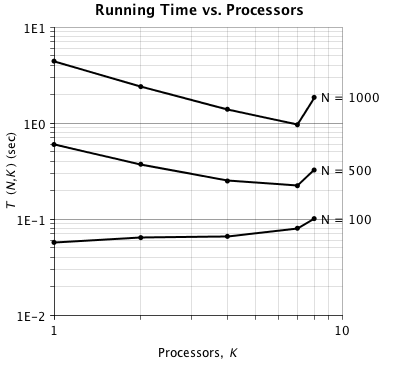
\includegraphics[scale=0.5]{images/matrix-inversion/running-vs-proc.png}
\end{center}
\begin{center}
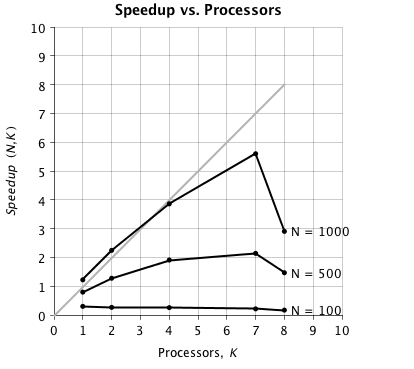
\includegraphics[scale=0.5]{images/matrix-inversion/speedup-vs-proc.png}
\end{center}
\begin{center}
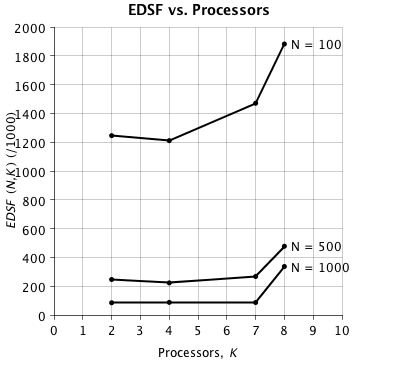
\includegraphics[scale=0.5]{images/matrix-inversion/edsf-vs-proc.png}
\end{center}
\begin{center}
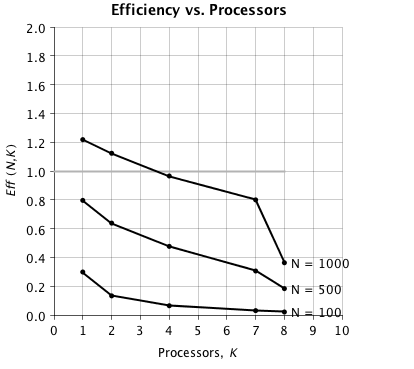
\includegraphics[scale=0.5]{images/matrix-inversion/eff-vs-proc.png}
\end{center}

\section{Conclusions}

While we did blah, blah, blah and blah, blah, we recognize that blah is blah. For further development, we would need to implement blah blah blah. However, with regard to the library in its current state, we are satisfied with blah and would like to continue to blah.

\newpage

\newpage
%
% The following two commands are all you need in the
% initial runs of your .tex file to
% produce the bibliography for the citations in your paper.
\bibliographystyle{abbrv}
\bibliography{bibliography}  % sigproc.bib is the name of the Bibliography in this case
% You must have a proper ".bib" file
%  and remember to run:
% latex bibtex latex
% to resolve all references
%
% ACM needs 'a single self-contained file'!
%
%APPENDICES are optional
\balancecolumns
% That's all folks!
\end{document}
